\documentclass[12pt, a4paper]{article}
\usepackage[left=2cm, right=2cm, top=2cm, bottom=2cm]{geometry}
\usepackage{graphicx}
\usepackage[colorlinks, urlcolor=blue]{hyperref}
\usepackage{xeCJK}

\setCJKmainfont{新細明體}

\title{
  Network Administration/System Administration\\
  (NTU CSIE, Spring 2024)\\
  Homework \#0
}
\author{\Large B12902110 呂承諺}
\date{}

\begin{document}
  \maketitle
  \section*{Network Administration}
  \section{True/False}
  \begin{enumerate}
    \item \textbf{True}. A VPN creates an encrypted tunnel between you and the
      VPN service provider. All of your internet traffic is routed to the VPN
      server first and then reach other sites, so it looks like you're connected
      to the internet from the VPN server. Sites will see the VPN server's IP
      address instead.

      References:
      \begin{itemize}
        \item \href{https://www.mcafee.com/learn/what-is-a-vpn-and-can-it-hide-my-ip-address/}{What is a VPN and Can it Hide My IP Address? | McAfee}
      \end{itemize}

    \item \textbf{False}. With techniques such as port forwarding or protocols
      such as the Port Control Protocol (PCP), and proper support from the NAT
      device, we can still actively initiate connections to internal devices
      behind the NAT.

      References:
      \begin{itemize}
        \item \href{https://en.wikipedia.org/wiki/Network_address_translation}{Network address translation - Wikipedia}
        \item \href{https://en.wikipedia.org/wiki/NAT_traversal}{NAT traversal - Wikipedia}
        \item \href{https://en.wikipedia.org/wiki/Port_Control_Protocol}{Port Control Protocol - Wikipedia}
        \item \href{https://en.wikipedia.org/wiki/Port_forwarding}{Port forwarding - Wikipedia}
      \end{itemize}

    \item \textbf{False}. Software such as pfSense can be used to implement
      gateways. Besides routing packets, a gateway can also provide services
      like NAT or DHCP. A gateway usually connects LAN and WAN, and it ensures
      that data are correctly transmitted.

      References:
      \begin{itemize}
        \item \href{https://en.wikipedia.org/wiki/PfSense}{pfSense - Wikipedia}
        \item \href{https://en.wikipedia.org/wiki/Gateway_(telecommunications)}{Gateway (telecommunications) - Wikipedia}
      \end{itemize}

    \item \textbf{True}. This site uses HTTP instead of HTTPS, so data is
      transmitted in plain text, including the submitted HTML form.

      References:
      \begin{itemize}
        \item \href{https://en.wikipedia.org/wiki/HTTP}{HTTP - Wikipedia}
        \item \href{https://en.wikipedia.org/wiki/HTML_form}{HTML form - Wikipedia}
      \end{itemize}

    \item \textbf{False}. It may be possible without DNS, but it is impossible
      to directly connect to the server without NAT because the client only
      has a private IP, which is not in the same subnet as the server.

    \item \textbf{False}. A DDoS attack is an attempt to kill a service by
      sending a lot of traffic to it. It could be defended by firewalls or
      traffic monitoring.

      References:
      \begin{itemize}
        \item \href{https://www.cloudflare.com/learning/ddos/what-is-a-ddos-attack/}{What is a distributed denial-of-service (DDoS) attack? | Cloudflare}
        \item \href{https://en.wikipedia.org/wiki/Denial-of-service_attack}{Denial-of-service attack - Wikipedia}
      \end{itemize}

    \item \textbf{False}. Triple DES is an counterexample. It has a mode
      that uses 168-bit keys, but due to the meet-in-the-middle attack,
      it only has 112 bits worth of effective security.

      References:
      \begin{itemize}
        \item \href{https://en.wikipedia.org/wiki/Triple_DES}{Triple DES - Wikipedia}
        \item My friend 黃昱翔 gave me an idea of this.
      \end{itemize}
  \end{enumerate}

  \section{ChatGPT}
  \begin{enumerate}
    \item Only partially correct.
    \begin{enumerate}
      \item Every network interface controller (NIC) has a hardcoded MAC
        address that cannot be changed, this is true.
      \item Although the hardware MAC address cannot be changed, many drivers
        allow the MAC address to be changed in software.\\
        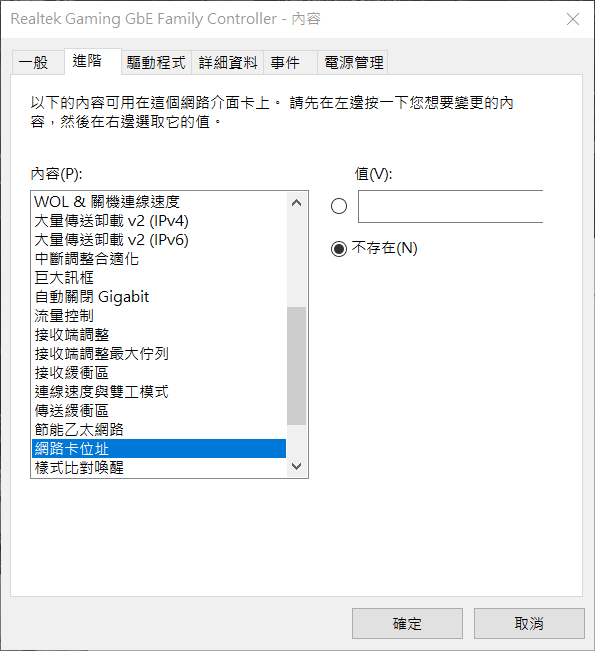
\includegraphics[width=0.5\textwidth]{na_p2-1_driver_mac_address.png}
      \item We could in theory completely rely on MAC addresses to identify
        devices on the internet, as a typical MAC address contains 48 bits,
        making random clashes extremely rare. However, this could reduce
        configurability. For example, we now use IP addresses and subnet masks
        to conveniently configure subnets, but if we use MAC addresses instead,
        we would have to maintain an exhaustive list of MAC addresses for every
        device in the subnet.
      \item Besides, if a ``device" has multiple NICs installed, it can have
        multiple MAC addresses, one per NIC.
    \end{enumerate}

    References:
    \begin{itemize}
      \item \href{https://en.wikipedia.org/wiki/MAC_spoofing}{MAC spoofing - Wikipedia}
      \item \href{https://www.quora.com/Can-you-change-the-MAC-address-of-a-network-card}{Can you change the MAC address of a network card? - Quora}
      \item \href{https://en.wikipedia.org/wiki/MAC_address}{MAC address - Wikipedia}
    \end{itemize}

    \item Mostly incorrect at first, totally incorrect at the end.
    \begin{itemize}
      \item 4G is a cellular network technology \textit{generation}, consisting
        of various standards. In these standards, some specify the frequency
        bands to be used, and others define thresholds for data speeds. So we
        wouldn't say 4G is a data speed nor say it's a frequency.
      \item We usually use $c$ to denote the speed of light in vacuum.
    \end{itemize}

    References:
    \begin{itemize}
      \item \href{https://en.wikipedia.org/wiki/4G}{4G - Wikipedia}
      \item \href{https://en.wikipedia.org/wiki/LTE_frequency_bands}{LTE frequency bands - Wikipedia}
      \item \href{https://en.wikipedia.org/wiki/Speed_of_light}{Speed of light - Wikipedia}
    \end{itemize}

    \item Mostly correct.
    \begin{enumerate}
      \item It's true that IPv4 uses 32 bits to represent an address, and that
        it has already faced the problem of address exhaustion. However, this
        means that all blocks of available IPv4 addresses have been assigned,
        and there may still be unused addresses in many of the blocks. Plus,
        we can recycle unused addresses and reuse them, so its not mandatory
        for new devices to use IPv6.
      \item There are still plenty of services that only support IPv4, so new
        devices still need IPv4 connectivity in order to access those services.
      \item Another thing is that IPv4 is usually more convenient to configure
        and sufficient in LANs. Anyway, IPv4 is still and will continue to be
        widely in use.
      \item It's correct that IPv6 uses 128 bits to represent an address.
    \end{enumerate}

    References:
    \begin{itemize}
      \item \href{https://en.wikipedia.org/wiki/Internet_Protocol_version_4}{Internet Protocol version 4 - Wikipedia}
      \item \href{https://en.wikipedia.org/wiki/IPv4_address_exhaustion}{IPv4 address exhaustion - Wikipedia}
      \item \href{https://en.wikipedia.org/wiki/IPv6}{IPv6 - Wikipedia}
    \end{itemize}
  \end{enumerate}

  \section{Short Answer}
  \begin{enumerate}
    \item
    \begin{enumerate}
      \item \textbf{DHCP}: Dynamic Host Configuration Protocol. An
        application-layer protocol that can automatically assign network
        configurations, such as IP addresses, subnet masks, and default
        gateways, to devices.
      \item \textbf{VLAN}: Virtual Local Area Network. A technology that groups
        devices so that they appear as if they are in their own network segment,
        even if they're connected to the same physical network. Can enhance
        performance or security.
      \item \textbf{Switch}: A network device that (usually) operates on the
        data link layer. It connects devices together and transmit network
        packets to the correct device by identifying the packet's destination
        MAC address.
      \item \textbf{Broadcast storm}: Broadcasting means sending a packet that
        will be received by every device in a given network. A broadcast strom
        happens when too many broadcast or multicast packets are flooding the
        network. This can happen if a switching loop exists in the network.
    \end{enumerate}
    References:
    \begin{itemize}
      \item \href{https://en.wikipedia.org/wiki/Dynamic_Host_Configuration_Protocol}{Dynamic Host Configuration Protocol - Wikipedia}
      \item \href{https://en.wikipedia.org/wiki/VLAN}{VLAN - Wikipedia}
      \item \href{https://en.wikipedia.org/wiki/Network_switch}{Network switch - Wikipedia}
      \item \href{https://en.wikipedia.org/wiki/Broadcast_storm}{Broadcast storm - Wikipedia}
      \item \href{https://en.wikipedia.org/wiki/Broadcasting_(networking)}{Broadcasting (networking) - Wikipedia}
      \item \href{https://en.wikipedia.org/wiki/Switching_loop}{Switching loop - Wikipedia}
    \end{itemize}

    \item These are all valid IPv4 addresses but reserved for special purposes.
    \begin{enumerate}
      \item Address block \verb|0.0.0.0/8| is reserved for \textit{this network}
        in software.
      \item The address \verb|::1| is reserved for the \textit{loopback
        address}, which loops any traffic back to the host itself.
      \item Address block \verb|2001:db8::/32| is reserved for use in
        documentation and example code.
    \end{enumerate}
    References:
    \begin{itemize}
      \item \href{https://en.wikipedia.org/wiki/Reserved_IP_addresses}{Reserved IP addresses - Wikipedia}
    \end{itemize}

    \item The 5 layers from top to bottom are:
    \begin{enumerate}
      \item \textbf{Application layer}: This layer includes protocols that
        applications use to exchange data between each other, such as SSH
        and HTTPS.
      \item \textbf{Transport layer}: This layer determines how to devices
        communicate and transfer data. TCP and UDP are the two primary protocols
        here.
      \item \textbf{Internet layer}: This layer is responsible for routing
        network packets across networks. IPv4 and IPv6 are protocols of this
        layer.
      \item \textbf{Link layer}: This layer includes protocols that operate
        on nodes of the local network segment (link), such as the Address
        Resolution Protocol (ARP). Network traffic in this layer is not
        routed to other networks.
      \item \textbf{Physical layer}: This layer handles the physical
        transmission of data through a medium, including electrical and
        mechanical specifications, such as 1000BASE-T and the physical part of
        IEEE 802.11.
    \end{enumerate}
    References:
    \begin{itemize}
      \item \href{https://www.ibm.com/docs/en/aix/7.3?topic=protocol-tcpip-protocols}{TCP/IP protocols - IBM Documentation}
      \item \href{https://en.wikipedia.org/wiki/Internet_protocol_suite}{Internet protocol suite - Wikipedia}
      \item \href{https://en.wikipedia.org/wiki/Transport_layer}{Transport layer - Wikipedia}
      \item \href{https://en.wikipedia.org/wiki/Internet_layer}{Internet layer - Wikipedia}
      \item \href{https://en.wikipedia.org/wiki/Link_layer}{Link layer - Wikipedia}
      \item \href{https://en.wikipedia.org/wiki/Physical_layer}{Physical layer - Wikipedia}
    \end{itemize}

    \item
    \begin{enumerate}
      \item \textbf{TCP}: An internet protocol in the transport layer that
        transfers data reliably and in order. A connection has to be established
        between the client and the server before data transmission can begin. It
        utilizes acknowledgements, data retransmission, etc. to ensure
        correctness of data.
      \item \textbf{UDP}: An internet protocol in the transport layer that
        transfers data less reliably. It is connectionless and doesn't guarantee
        correctness of data.
      \item TCP:
        \begin{itemize}
          \item Advantages: More reliable.
          \item Disadvantages: Higher latency.
          \item Example: When we \textit{SSH} into CSIE's workstation.
        \end{itemize}
        UDP:
        \begin{itemize}
          \item Advantages: Lower latency, useful for time-critical applications.
          \item Disadvantage: Less reliable.
          \item Example: When we perform a \textit{DNS} query.
        \end{itemize}
    \end{enumerate}
    References:
    \begin{itemize}
      \item \href{https://en.wikipedia.org/wiki/Transmission_Control_Protocol}{Transmission Control Protocol - Wikipedia}
      \item \href{https://en.wikipedia.org/wiki/User_Datagram_Protocol}{User Datagram Protocol - Wikipedia}
      \item \href{https://www.avast.com/c-tcp-vs-udp-difference}{TCP vs UDP: Differences Between TCP \& UDP Protocols | Avast}
    \end{itemize}

    \item
    \begin{enumerate}
      \item \textbf{LDAP/LDAPS}: Lightweight Directory Access Protocol/LDAP over SSL
      \begin{itemize}
        \item Manage directory information services over IP.
        \item A directory contains information of objects like users, groups,
          and devices. A common use of this protocol is maintaining a
          centralized storage of user credentials.
        \item LDAPS is essentially LDAP with encryption.
        \item Default port: 389 for LDAP, 636 for LDAPS.
      \end{itemize}

      \item \textbf{SMTP}: Simple Mail Transfer Protocol
      \begin{itemize}
        \item Send emails over the internet.
        \item Default port: 465, 587, or traditionally 25.
      \end{itemize}

      \item \textbf{SNMP}: Simple Network Management Protocol
      \begin{itemize}
        \item Monitor and manage devices in an IP network.
        \item Gather system status information and configure settings remotely.
        \item Default port: 161 and 162.
      \end{itemize}

       \item \textbf{HTTP/HTTPS}: Hypertext Transfer Protocol/HTTP over SSL
       \begin{itemize}
         \item Transfer hypermedia resources, such as HTML.
         \item HTTPS is HTTP with encryption.
         \item Default port: 80 for HTTP, 443 for HTTPS.
       \end{itemize}
    \end{enumerate}
    References:
    \begin{itemize}
      \item \href{https://en.wikipedia.org/wiki/Lightweight_Directory_Access_Protocol}{Lightweight Directory Access Protocol - Wikipedia}
      \item \href{https://en.wikipedia.org/wiki/Simple_Mail_Transfer_Protocol}{Simple Mail Transfer Protocol - Wikipedia}
      \item \href{https://en.wikipedia.org/wiki/Simple_Network_Management_Protocol}{Simple Network Management Protocol - Wikipedia}
      \item \href{https://developer.mozilla.org/en-US/docs/Web/HTTP}{HTTP | MDN}
      \item \href{https://en.wikipedia.org/wiki/HTTPS}{HTTPS - Wikipedia}
    \end{itemize}
  \end{enumerate}

  \section{Command Line Utilities}
  \begin{enumerate}
    \item To find the IP addresses of the domain names, we run
      \verb|dig DOMAIN_NAME| to perform DNS queries.
      \begin{enumerate}
        \item www.ntu.etu.tw \textrightarrow\ 140.112.8.116
        \item csie.ntu.edu.tw \textrightarrow\ 140.112.30.26
      \end{enumerate}
      To find the domain names IP addresses, we run
      \verb|dig -x ADDRESS| to perform reverse DNS lookup queries.
      \begin{enumerate}
        \item 140.112.30.25 \textrightarrow\ printing.csie.ntu.edu.tw
        \item 140.112.161.176 \textrightarrow\ if176.aca.ntu.edu.tw
      \end{enumerate}

      References:
      \begin{itemize}
        \item \href{https://serverfault.com/questions/7056/whats-the-reverse-dns-command-line-utility}{linux - What's the reverse DNS command line utility? - Server Fault}
        \item man page of \verb|dig|
      \end{itemize}

    \item NTU VPN
    \begin{enumerate}
      \item 140.112.77.110. We can see this in the VPN client software or
        Windows control panel details.\\
        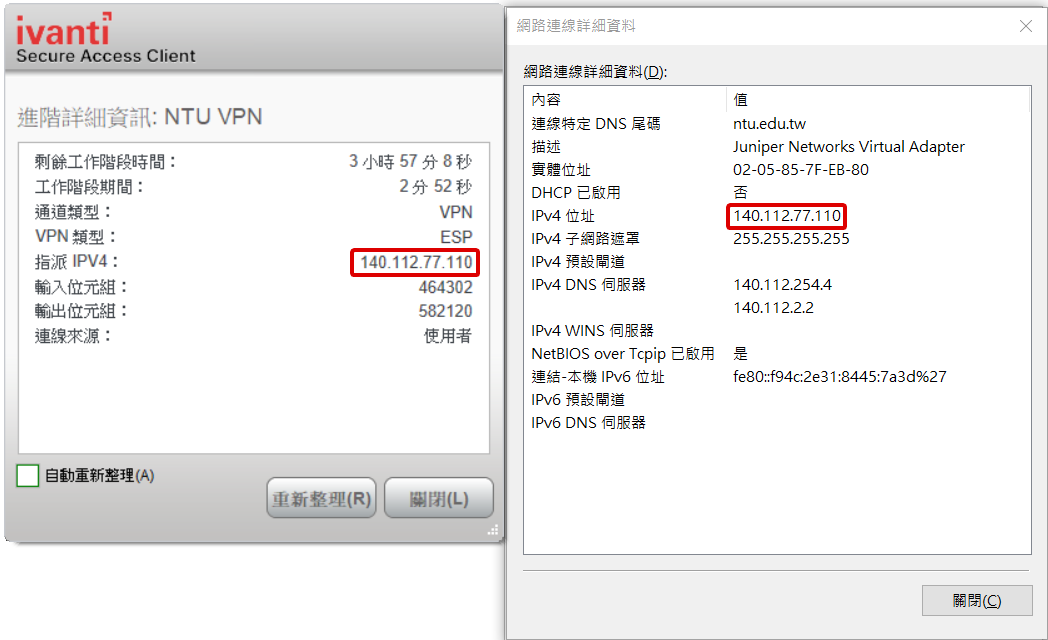
\includegraphics[width=0.75\textwidth]{na_p4-2_ntu_vpn_ip.png}
      \item We use \verb|nslookup| to query IPs and use \verb|tracert| to find
        out the route.

        Before connecting to VPN (using Wi-Fi ntu\_peap):
        \begin{itemize}
          \item DNS server IP: 140.112.254.4
          \item Route to DNS server: refer to the figure below
        \end{itemize}
        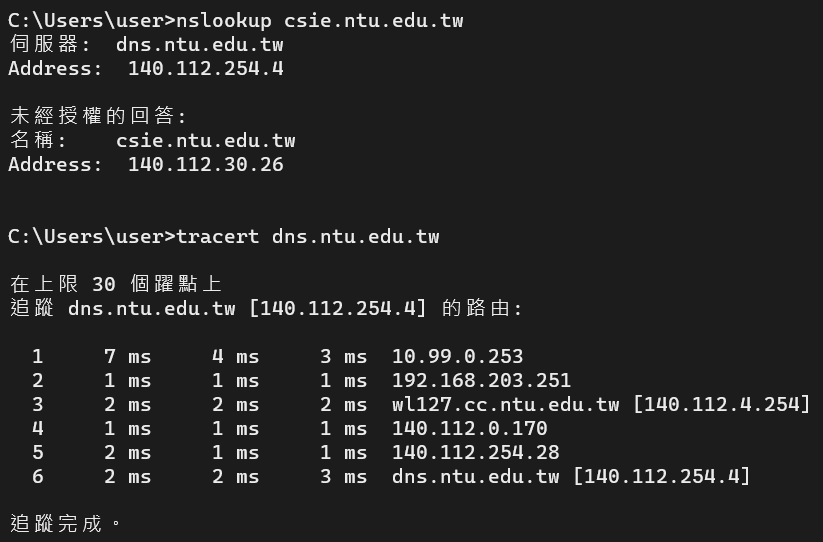
\includegraphics[width=0.65\textwidth]{na_p4-2_dns_query_and_route.png}\\
        After connecting to VPN:
        \begin{itemize}
          \item DNS server IP: 140.112.254.4
          \item Route to DNS server: refer to the figure below
        \end{itemize}
        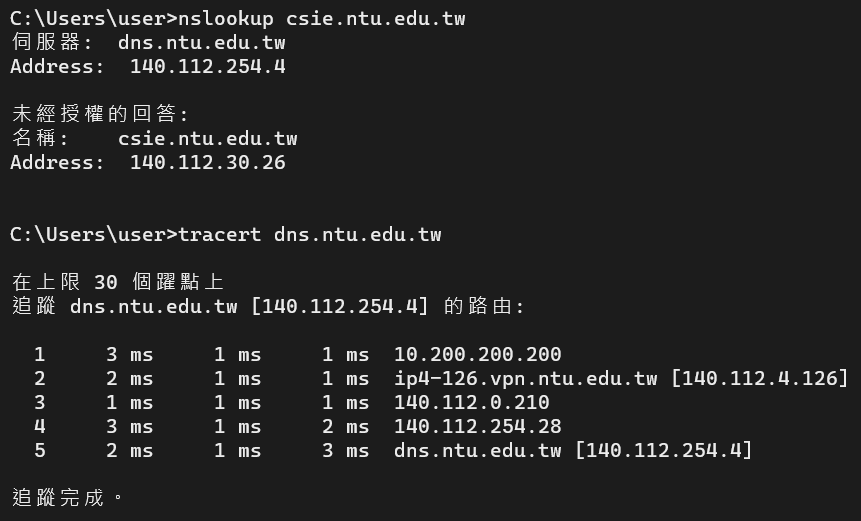
\includegraphics[width=0.65\textwidth]{na_p4-2_dns_query_and_route_vpn.png}

      \item Run \verb|nmap 140.112.30.158 -p-| to scan for all open ports.\\
        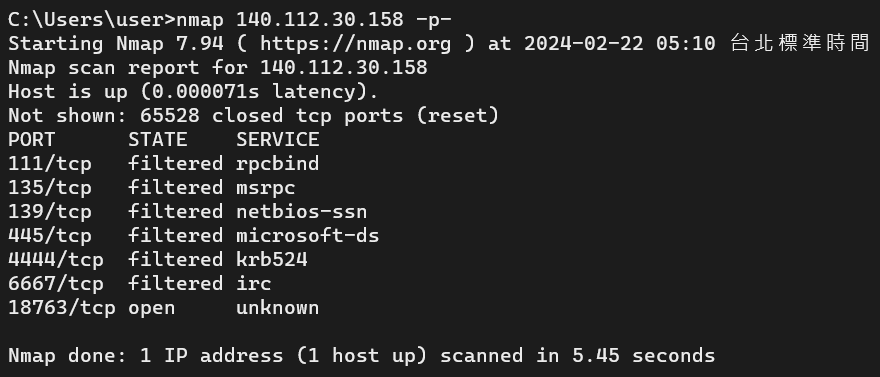
\includegraphics[width=0.8\linewidth]{na_p4-3_nmap.png}\\
        Run \verb|nc 140.112.30.158 18763| to see the message.\\
        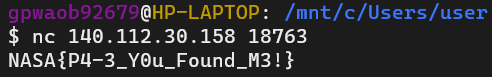
\includegraphics[width=0.5\textwidth]{na_p4-3_nc.png}

        References:
        \begin{itemize}
          \item \href{https://linuxize.com/post/check-open-ports-linux/}{How to Check (Scan) for Open Ports in Linux | Linuxize}
        \end{itemize}
    \end{enumerate}
  \end{enumerate}

  \clearpage
  \section*{System Administration}
  \setcounter{section}{0}
  \section{Super Auto Penguin!}
  \paragraph{Steps}
  \begin{enumerate}
    \item Login with the provided credentials.
    \item Run \verb|sudo ./p1-checker|. We can see the flag in standard output.
  \end{enumerate}
  \paragraph{Flag} \verb|NASA{P1_I_4m_r00t!}|

  \section{Read the manual plz}
  \paragraph{Steps}
  \begin{enumerate}
    \item Run \verb|man pacman|.
    \item We discover the flag at the end of the first paragraph of the
      \textit{DESCRIPTION} section.
  \end{enumerate}
  \paragraph{Flag} \verb|NASA{P2_P4CM4N_1$_TH3_M4N}|

  \section{Telepathy}
  \paragraph{Steps}
  \begin{enumerate}
    \item Run \verb|sudo pacman -Sy openssh|. The package
      \verb|openssh-9.6p1-1| is updated to\\ \verb|openssh-9.6p1-3|.\\
      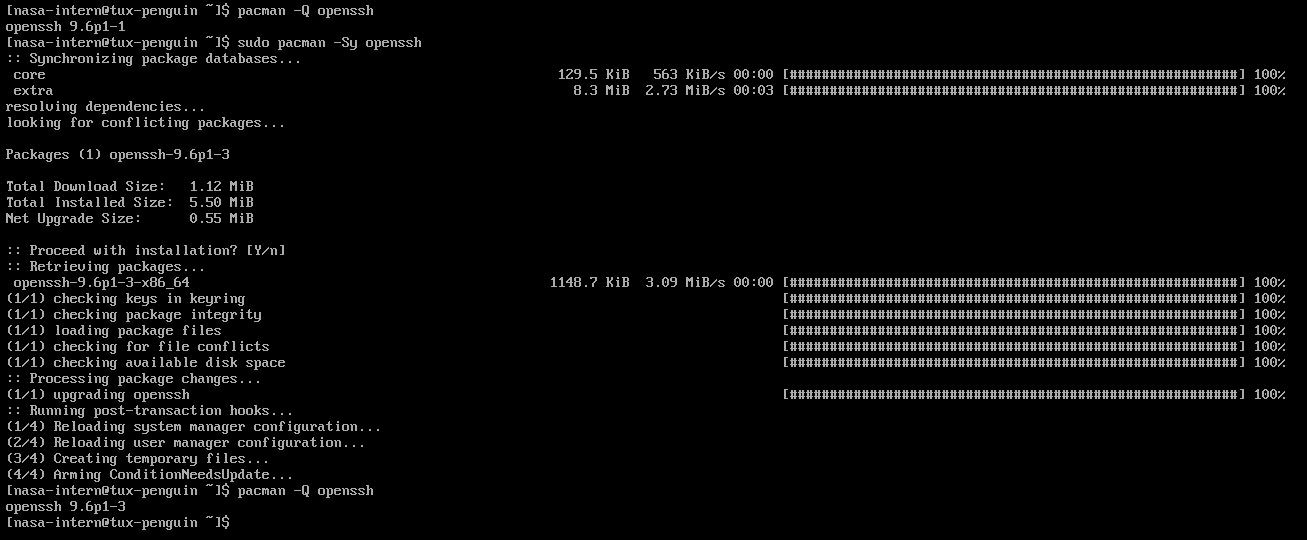
\includegraphics[width=0.9\textwidth]{sa_p2_openssh_upgrade.png}
    \item Run \verb|sudo systemctl start sshd| to start the \verb|openssh|
      service.
    \item Run \verb|ip addr| to get the IP address of the virtual machine.
      In my case its \verb|192.168.15.138|.\\
      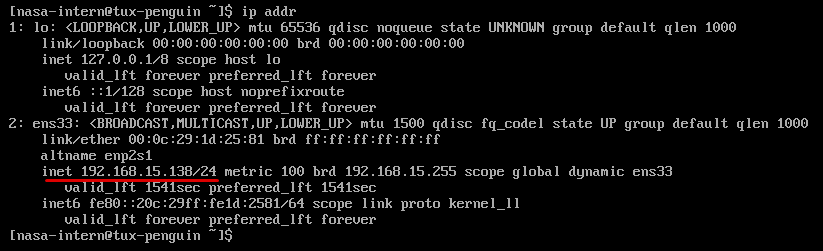
\includegraphics[width=0.9\textwidth]{sa_p2_ip.png}
    \item Run \verb|ssh 192.168.15.138| on the host machine and login.
      (I'm using VMWare workstation.)\\
      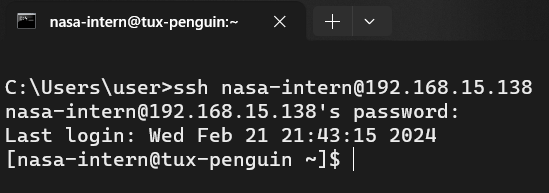
\includegraphics[width=0.6\linewidth]{sa_p2_ssh_login.png}
  \end{enumerate}
  \paragraph{References}
  \begin{itemize}
    \item \href{https://wiki.archlinux.org/title/pacman}{pacman - ArchWiki}
    \item \href{https://unix.stackexchange.com/questions/13073/update-only-one-package-with-pacman}{arch linux - Update only one package with pacman - Unix \& Linux Stack Exchange}
    \item \href{https://wiki.archlinux.org/title/systemd}{systemd - ArchWiki}
    \item \href{https://superuser.com/questions/1229344/is-there-any-linux-command-that-i-can-use-to-show-all-the-network-interfaces-exc}{Is there any Linux command that I can use to show all the network interfaces except ifconfig - Super User}
  \end{itemize}

  \section{Sudden Airdrop?}
  \paragraph{Steps}
  \begin{enumerate}
    \item Run \verb|unzip airdrop.tar.gz.zip| to get \verb|airdrop.tar.gz|.
    \item Run \verb|tar xzf airdrop.tar.gz| to get the \verb|airdrop| folder.
    \item Navigate through \verb|~/airdrop| with commands
      \verb|cd| and \verb|ls -al|. We reach \verb|~/airdrop/p4| and discover
      a file named \verb|flag|.
    \item Run \verb|cat flag| to obtain the flag.
      (Working directory: \verb|~/airdrop/p4|)
  \end{enumerate}
  \paragraph{Flag} \verb|NASA{P4_Matryoshka_Files}|
  \paragraph{References}
  \begin{itemize}
    \item \href{https://askubuntu.com/questions/86849/how-to-unzip-a-zip-file-from-the-terminal}{command line - How to unzip a zip file from the Terminal? - Ask Ubuntu}
    \item \href{https://stackoverflow.com/questions/651018/opening-a-tar-gz-file-with-a-single-command}{linux - Opening a .tar.gz file with a single command - Stack Overflow}
  \end{itemize}

  \section{Shifting Identity}
  \paragraph{Steps}
  \begin{enumerate}
    \item Run \verb|sudo nano /etc/hostname| and change the hostname to
      \verb|totally-not-tux|.
    \item Run \verb|sudo reboot| to reboot the system.\\
      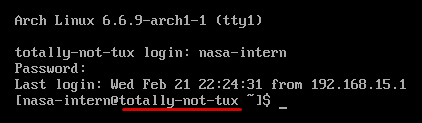
\includegraphics[width=0.6\linewidth]{sa_p5_hostname_changed.png}
    \item Run \verb|sudo usermod -c "Definitely Legit Guy" nasa-intern| to
      change the full name of this account.
    \item Run \verb|./security| to obtain the flag.
      (Working directory: \verb|~/airdrop|)
  \end{enumerate}
  \paragraph{Flag} \verb|NASA{P5_Th3_5PY_1s_Am0nG_U5}|
  \paragraph{References}
  \begin{itemize}
    \item \href{https://magiclen.org/linux-change-hostname/}{如何更改Linux作業系統的主機名稱(hostname)? | MagicLen}
    \item \href{https://unix.stackexchange.com/questions/149665/change-user-info-on-the-command-line}{Change user info on the command line - Unix \& Linux Stack Exchange}
  \end{itemize}

  \section{DIY Friendship}
  \paragraph{Steps}
  \begin{enumerate}
    \item Run \verb|sudo useradd coolguy|.
    \item Run \verb|sudo groupadd friends|.
    \item Run \verb|sudo usermod -aG friends nasa-intern| and
      \verb|sudo usermod -aG friends coolguy|.
    \item Run \verb|./friendship-test| to obtain the flag.
      (Working directory: \verb|~/airdrop/p6|)
  \end{enumerate}
  \paragraph{Flag} \verb|NASA{P6_W3_4r3_fri3nd5_n0t_f00d}|
  \paragraph{References}
  \begin{itemize}
    \item \href{https://www.redhat.com/sysadmin/linux-groups}{How to create, delete, and modify groups in Linux | Enable Sysadmin}
  \end{itemize}

  \section{Access Denied}
  \paragraph{Steps}
  \begin{enumerate}
    \item Run \verb|chmod 710 p7|. (Working directory: \verb|~/airdrop|)
    \item Run \verb|./pentester| to obtain the flag.
      (Working directory: \verb|~/airdrop/p7|)
  \end{enumerate}
  \paragraph{Flag} \verb|NASA{P7_I5_th1s_TH3_h0m3w0rk_f0ld3er?}|
  \paragraph{References}
  \begin{itemize}
    \item \href{https://en.wikipedia.org/wiki/Chmod}{chmod - Wikipedia}
    \item \href{https://serverfault.com/questions/428885/how-are-r-directory-permissions-supposed-to-work-on-linux}{How are r-- directory permissions supposed to work on Linux? - Server Fault}
  \end{itemize}

  \section{Careless Cool Cat Commentator}
  \paragraph{Steps}
  Consult \verb|cowsay|'s man page and run \verb|ls /usr/share/cows| to search
  for the most likely cowfile to use. \verb|cow-and-dragon| seems to be it.
  \paragraph{Flag}
  \begin{itemize}
    \item Black and white: \verb|NASA{P8_cowsay -f dragon-and-cow "Hello there!"}|
    \item Rainbow color: \begin{verbatim}NASA{P8_cowsay -f dragon-and-cow "My name is RTX 4090" | lolcat}\end{verbatim}
  \end{itemize}
  \paragraph{References}
  \begin{itemize}
    \item \href{https://schier.co/blog/add-colorful-cows-to-your-terminal}{Add Colorful Cows to Your Terminal – Gregory Schier}
    \item man page of \verb|cowsay| and \verb|lolcat|
    \item I overheard my friend 李承瑜 saying ``cowsay".
  \end{itemize}

  \section{Careless Cool Cat Commentator}
  \paragraph{Steps} Run:
  \begin{verbatim}
sed s/gentoo//g book |
  tr "aFS9PoUYXyQEvDfc7bVqW5hg)s18NeziB6xt0(RJjumM{Zkw3d4CGnT}rOLKH2lpAI"
    "abcdefghijklmnopqrstuvwxyzABCDEFGHIJKLMNOPQRSTUVWXYZ0123456789(){}" |
  grep NASA
  \end{verbatim}
  (Working directory: \verb|~/airdrop/p9|)
  \paragraph{Flag} \verb|NASA{P9_I_Prefer_Arch}|
  \paragraph{References}
  \begin{itemize}
    \item \href{https://unix.stackexchange.com/questions/159367/using-sed-to-find-and-replace}{shell script - Using 'sed' to find and replace - Unix \& Linux Stack Exchange}
    \item man page of \verb|sed|, \verb|tr|, and \verb|grep|
  \end{itemize}

  \section{Directory Maze}
  \paragraph{Steps}
  \begin{enumerate}
    \item Run \verb|find . -name '*NASA*'|.
      (Working directory: \verb|~/airdrop/p10|)
    \item We obtain the flag in
      \verb|./maze/W/A/E/NASA{P10_D0_Y0U_F1ND_DA_W43}|.
  \end{enumerate}
  \paragraph{Flag} \verb|NASA{P10_D0_Y0U_F1ND_DA_W43}|
  \paragraph{References}
  \begin{itemize}
    \item \href{https://blog.miniasp.com/post/2010/08/27/Linux-find-command-tips-and-notice}{在 Linux 下使用 find 指令查詢目錄與檔案的速查筆記 | The Will Will Web}
    \item man page of \verb|find|
  \end{itemize}

  \section{Loop de Loop}
  \paragraph{Steps}
  \begin{enumerate}
    \item
    \begin{enumerate}
      \item Run \verb|./loop|. (Working directory: \verb|~/airdrop/p11|)
      \item Press Ctrl + Z to suspend the program.
      \item Run \verb|fg| to resume the program and obtain the first flag.
    \end{enumerate}
    \item
    \begin{enumerate}
      \item Switch to tty2 by pressing Ctrl + Shift + F2.
      \item Run \verb|killall loop|.
      \item Switch back to tty1 and obtain the second flag.
    \end{enumerate}
    \item
    \begin{enumerate}
      \item Switch to tty2 and run \verb|killall -s SIGKILL loop|.
      \item Switch back to tty1 and confirm that the process has been killed.\\
        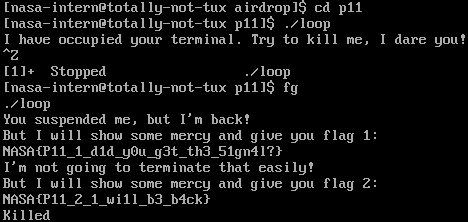
\includegraphics[width=0.9\linewidth]{sa_p11.png}
    \end{enumerate}
  \end{enumerate}
  \paragraph{Flag}
  \begin{enumerate}
    \item \verb|NASA{P11_1_d1d_y0u_g3t_th3_51gn4l?}|
    \item \verb|NASA{P11_2_1_wi1l_b3_b4ck}|
    \item \verb|NASA{P11_3_killall -s SIGKILL loop}|
  \end{enumerate}
  \paragraph{References}
  \begin{itemize}
    \item \href{https://stackoverflow.com/questions/27844970/how-to-pause-resume-a-process-in-linux}{vlc - How to Pause/Resume a process in Linux - Stack Overflow}
    \item \href{ https://unix.stackexchange.com/questions/167386/how-to-switch-between-tty-and-xorg-session}{linux - How to switch between tty and xorg session - Unix \& Linux Stack Exchange}
    \item \href{https://stackoverflow.com/questions/160924/how-can-i-kill-a-process-by-name-instead-of-pid-on-linux}{bash - How can I kill a process by name instead of PID, on Linux? - Stack Overflow}
    \item man page of \verb|killall|
    \item \href{https://man7.org/linux/man-pages/man7/signal.7.html}{signal(7) - Linux manual page}
  \end{itemize}

  \section{The Final Showdown}
  \paragraph{Steps}
  \begin{enumerate}
    \item
    \begin{enumerate}
      \item Run \verb|command -v vim|, which outputs \verb|alias vim='nano'|.
        We suspect that code somewhere is setting suspicious bash aliases.
      \item Run \verb|nano ~/.bashrc|, and we see some malicious aliases at
        lines 13 to 15.
      \item Remove those lines and re-login. Now \verb|vim| and \verb|vi| works.
    \end{enumerate}
    \item
    \begin{enumerate}
      \item But after tens of seconds, a strange message appears with a piece of
        ASCII art.
      \item With hints from the problem description and observations of system
        behavior, the message seems to appear every minute. After searching
        the internet, we suspect that a malicious task is scheduled to run
        every minute.
      \item Dive into \verb|/etc/cron.d| and inspect the file \verb|minute|.
        Here we see that line 5 is malicious:
        \verb|*/1 * * * * root /usr/src/nano_gang/check.sh|.
      \item Remove that line and re-login. Now the message and ASCII art no
        longer appears, and \verb|~/.bashrc| doesn't revert to the dirty
        version anymore.
    \end{enumerate}
  \end{enumerate}
  \paragraph{References}
  \begin{itemize}
    \item \href{https://debian-handbook.info/browse/en-US/stable/sect.task-scheduling-cron-atd.html}{9.7. Scheduling Tasks with cron and atd}
  \end{itemize}
\end{document}
